\section{L'atome de Fer}

\begin{multicols}{2}
	
	
	Le métal fer est un cristal, ce qui veut dire que ses atomes sont organisés selon une structure bien particulière appelée maille élémentaire. Sur l'Atomium à Bruxelles, chaque sphère de 18 m de diamètre représente un atome de fer agrandi 64 milliards de fois.
	
	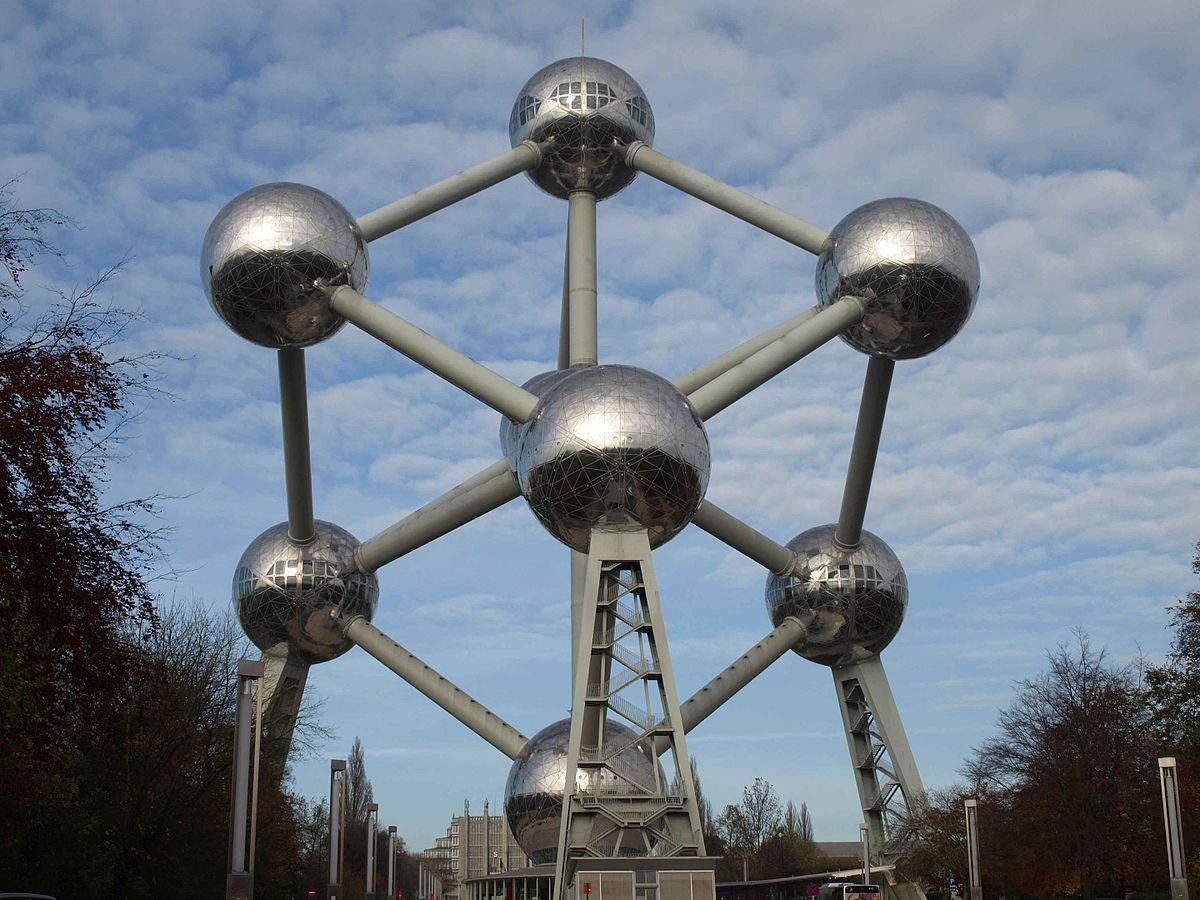
\includegraphics[scale=0.5]{img/atomium}
\end{multicols}


\begin{questions}
	\question Calculer le diamètre d'un atome de fer.
	\fillwithdottedlines{1.5cm}
	
	\question Combien d'électrons contient-il ?
	\fillwithdottedlines{1.5cm}
	
	\question Quel est le diamètre du noyau d'un atome de fer ?
	\fillwithdottedlines{1.5cm}
\end{questions}

